%
%Не забыть:
%--------------------------------------
%Вставить колонтитулы, поменять название на титульнике



%--------------------------------------

\documentclass[a4paper, 12pt]{article} 

%--------------------------------------
%Russian-specific packages
%--------------------------------------
%\usepackage[warn]{mathtext}
\usepackage[T2A]{fontenc}
\usepackage[utf8]{inputenc}
\usepackage[english,russian]{babel}
\usepackage[intlimits]{amsmath}
\usepackage{esint}
%--------------------------------------
%Hyphenation rules
%--------------------------------------
\usepackage{hyphenat}
\hyphenation{ма-те-ма-ти-ка вос-ста-нав-ли-вать}
%--------------------------------------
%Packages
%--------------------------------------
\usepackage{amsmath}
\usepackage{amssymb}
\usepackage{amsfonts}
\usepackage{amsthm}
\usepackage{latexsym}
\usepackage{mathtools}
\usepackage{etoolbox}%Булевые операторы
\usepackage{extsizes}%Выставление произвольного шрифта в \documentclass
\usepackage{geometry}%Разметка листа
\usepackage{indentfirst}
\usepackage{wrapfig}%Создание обтекаемых текстом объектов
\usepackage{fancyhdr}%Создание колонтитулов
\usepackage{setspace}%Настройка интерлиньяжа
\usepackage{lastpage}%Вывод номера последней страницы в документе, \lastpage
\usepackage{soul}%Изменение параметров начертания
\usepackage{hyperref}%Две строчки с настройкой гиперссылок внутри получаеммого
\usepackage[usenames,dvipsnames,svgnames,table,rgb]{xcolor}% pdf-документа
\usepackage{multicol}%Позволяет писать текст в несколько колонок
\usepackage{cite}%Работа с библиографией
\usepackage{subfigure}% Человеческая вставка нескольких картинок
\usepackage{tikz}%Рисование рисунков
\usetikzlibrary{circuits} % подключаем библиотеки, содержащие
\usetikzlibrary{circuits.ee} % УГО для схем
\usetikzlibrary{circuits.ee.IEC}
\usetikzlibrary{arrows} % подключаем библиотеки со стрелками
\usetikzlibrary{patterns} % и со штриховкой
\usepackage{float}% Возможность ставить H в положениях картинки
% Для картинок Моти
\usepackage{misccorr}
\usepackage{lscape}
\usepackage{cmap}
\usepackage{bm}
\newtheorem{definition}{Опредление}



\usepackage{graphicx,xcolor}
\graphicspath{{Pictures/}}
\DeclareGraphicsExtensions{.pdf,.png,.jpg}

%----------------------------------------
%Список окружений
%----------------------------------------
\newenvironment {theor}[2]
{\smallskip \par \textbf{#1.} \textit{#2}  \par $\blacktriangleleft$}
{\flushright{$\blacktriangleright$} \medskip \par} %лемма/теорема с доказательством
\newenvironment {proofn}
{\par $\blacktriangleleft$}
{$\blacktriangleright$ \par} %доказательство
%----------------------------------------
%Список команд
%----------------------------------------
\newcommand{\grad}
{\mathop{\mathrm{grad}}\nolimits\,} %градиент

\newcommand{\diver}
{\mathop{\mathrm{div}}\nolimits\,} %дивергенция

\newcommand{\rot}
{\ensuremath{\mathrm{rot}}\,}

\newcommand{\Def}[1]
{\underline{\textbf{#1}}} %определение

\newcommand{\RN}[1]
{\MakeUppercase{\romannumeral #1}} %римские цифры

\newcommand {\theornp}[2]
{\textbf{#1.} \textit{ #2} \par} %Написание леммы/теоремы без доказательства

\newcommand{\qrq}
{\ensuremath{\quad \Rightarrow \quad}} %Человеческий знак следствия

\newcommand{\const}{\text{const}} % Написание const в формулах

\newcommand{\qlrq}
{\ensuremath{\quad \Leftrightarrow \quad}} %Человеческий знак равносильности

\renewcommand{\phi}{\varphi} %Нормальный знак фи

\renewcommand{\epsilon}{\varepsilon}

\newcommand{\me}
{\ensuremath{\mathbb{E}}}

\newcommand{\md}
{\ensuremath{\mathbb{D}}}



%\renewcommand{\vec}{\overline}




%----------------------------------------
%Разметка листа
%----------------------------------------
\geometry{top = 3cm}
\geometry{bottom = 2cm}
\geometry{left = 1.5cm}
\geometry{right = 1.5cm}
%----------------------------------------
%Колонтитулы
%----------------------------------------
\pagestyle{fancy}%Создание колонтитулов
\fancyhead{}
%\fancyfoot{}
\fancyhead[R]{\textsc{Фотонные кристаллы}}%Вставить колонтитул сюда
%----------------------------------------
%Интерлиньяж (расстояния между строчками)
%----------------------------------------
%\onehalfspacing -- интерлиньяж 1.5
%\doublespacing -- интерлиньяж 2
%----------------------------------------
%Настройка гиперссылок
%----------------------------------------
\hypersetup{				% Гиперссылки
	unicode=true,           % русские буквы в раздела PDF
	pdftitle={Заголовок},   % Заголовок
	pdfauthor={Автор},      % Автор
	pdfsubject={Тема},      % Тема
	pdfcreator={Создатель}, % Создатель
	pdfproducer={Производитель}, % Производитель
	pdfkeywords={keyword1} {key2} {key3}, % Ключевые слова
	colorlinks=false,       	% false: ссылки в рамках; true: цветные ссылки
	linkcolor=blue,          % внутренние ссылки
	citecolor=blue,        % на библиографию
	filecolor=magenta,      % на файлы
	urlcolor=blue           % на URL
}
%----------------------------------------
%Работа с библиографией 
%----------------------------------------
\renewcommand{\refname}{Список литературы}%Изменение названия списка литературы для article
%\renewcommand{\bibname}{Список литературы}%Изменение названия списка литературы для book и report
%----------------------------------------
\begin{document}
	\begin{titlepage}
		\begin{center}
			$$$$
			$$$$
			$$$$
			$$$$
			{\Large{НАЦИОНАЛЬНЫЙ ИССЛЕДОВАТЕЛЬСКИЙ УНИВЕРСИТЕТ}}\\
			\vspace{0.1cm}
			{\Large{ВЫСШАЯ ШКОЛА ЭКОНОМИКИ}}\\
			\vspace{0.25cm}
			{\large{Факультет физики}}\\
			\vspace{5.5cm}
			{\Huge\textbf{{Отчёт}}}\\%Общее название
			\vspace{1cm}
			{\LARGE{<<Фотонные кристаллы>>}}\\%Точное название
			\vspace{1cm}
			{\LARGE{Блуменау М. И.}}\\%Лектор
			\vspace{2cm}
			\vfill
			
\includegraphics[width = 0.2\textwidth]{HSElogo}\\
			\vfill
			Москва\\
			2021
		\end{center}
	\end{titlepage}
	
	\tableofcontents
	\newpage
	\addcontentsline{toc}{section}{Введение}
	\section*{Введение}
	Целью данной работы являлось исследование необычных свойств фотонных кристаллов, а именно с переодическим изменением показателя преломления на масштабах сравнимых с длиной волны. В оптическом спектре фотонных кристаллов существуют узкие области длин волн, для которых распространение света подавляется. Такие необычные оптические свойства используются для создания разнообразных оптических элементов на основе фотонных кристаллов (оптических фильтров, отражателей).
	В данной работе свойства фотонных кристаллов изучались на примере пористых (содержащих воздушные каналы) пленок анодного оксида алюминия. Структура образцов, полученных с помощью электрохимического окисления (анодирования) алюминия, может быть представлена как система несвязанных цилиндрических каналов, расположенных перпендикулярно поверхности образца. На рисунке \ref{fig:1} изображена примерная структура вышеупомянутых цилиндрических каналов.
	\begin{figure}[H]
		\centering
		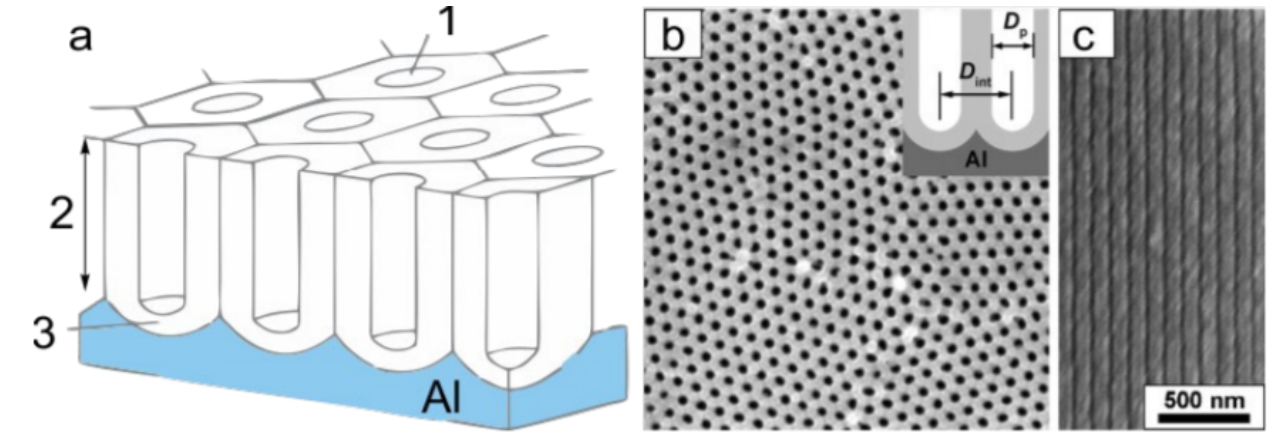
\includegraphics[width=1\linewidth]{Struct.png}
		\caption{(а) Схематическая структура пористой пленки оксида алюминия: 1 - пора, 2 - пористый слой, 3 - барьерный слой. Изображение пленки, полученное с помощью электронного микроскопа: (b) вид сверху, (с) поперечное.}
		\label{fig:1}
	\end{figure}
	\addcontentsline{toc}{section}{Теоретическая справка}
	\section*{Теоретическая справка}
	Рассмотрим параллельный монохроматический пучок с постоянной интенсивностью и длиной волны $\lambda$, падающий на фотонной кристалл. Пучки, отраженные от разных слоёв, интерферируют между собой. В результате интерференционная картина в отражённом свете имеет максимумы при определённых углах падения $\theta$ (минимумы пропускания наблюдаются при тех же углах), которые, согласно закону Брэга-Снелла, определяются условием:
	\begin{equation}\label{bg}
	2D\sqrt{n^{2}-\sin^{2}{\theta}}  =  m\lambda,
	\end{equation}
	где D период структуры фотонного кристалла, n - средний показатель преломления фотонного кристалла, $m= 1,2, ...$ – порядок интерференции, $\lambda$- длина волны света.
	
	Заранее линеаризуем данную формулу (возведя обе части в квадрат и перенеся необходимые слагаемые):
	\begin{equation}\label{linear}
	\sin^{2}{\phi}=\frac{4D^{2}n^{2}}{h^2}-\frac{4D^{2}}{h^{2}}\sin^{2}{\theta},
	\end{equation}
	где видно, что зависимость линейна относительна квадратов синусов.
	Также заранее запишем формулу, связывающую угол дифракции при
	прохождении дифракционной решётки $\phi$ и длину волны $\lambda$ :
	\begin{equation}\label{diflen}
	h\sin{\phi} = m\lambda
	\end{equation}
	\addcontentsline{toc}{section}{Оборудование и методы}
	\section*{Оборудование и методы}
	Список использованного оборудования: линза, фотонный кристалл, дифракционная решётка, красный лазер с длиной волны 660нм, фотодиод, мультиметр, батарейка типа "Крона" напряжением 9В. На рисунке \ref{fig:2} ниже изображена установка первой части работы.
	
	Для обработки результатов использовался язык программирования Python и совокупность пакетов Anaconda.
	Ссылка на исходный код:
	\newline \href{https://github.com/burunduk387/HSE-FF/tree/main/LabOptics/Фотонные\%20кристаллы}{https://github.com/burunduk387/HSE-FF/tree/main/LabOptics/Фотонные\%20кристаллы}
	\begin{figure}[H]
		\centering
		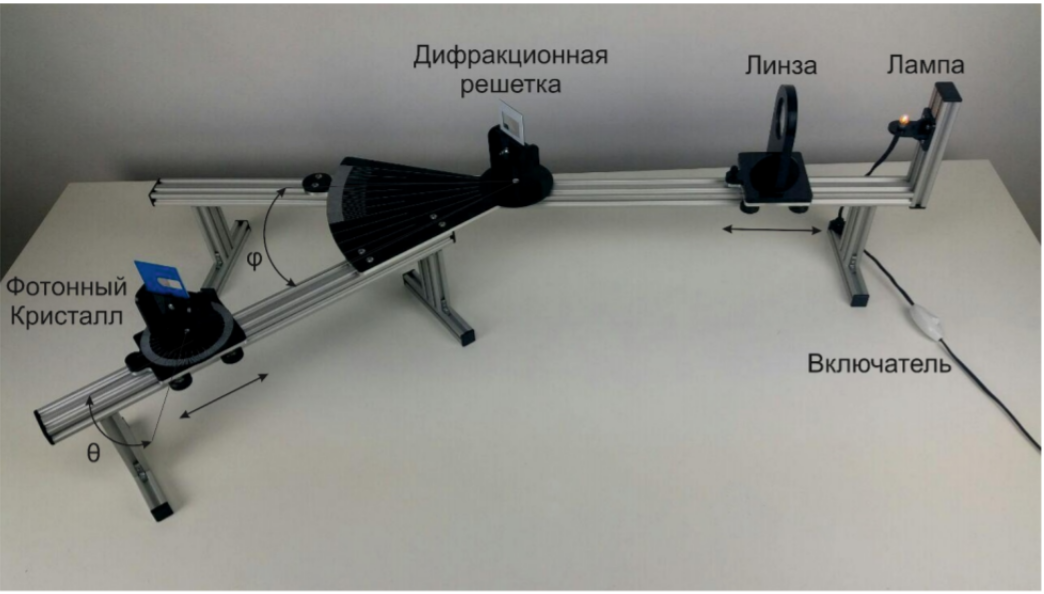
\includegraphics[width=1\linewidth]{Equip.png}
		\caption{Используемое оборудование в первой части эксперимента.}
		\label{fig:2}
	\end{figure}
	\addcontentsline{toc}{section}{Первый эксперимент}
	\section*{Первый эксперимент}
	На рисунке \ref{fig:3} изображена схема установки. Процесс выполнения работы таков: включаем лампочку и видим узкую полоску спектра на диффракционной решётке. Изменяя углы, подбираем их так, чтобы стала видна стоп-зона. Её достаточно просто увидеть. Тогда начнём изменять углы, следя за ней и стараясь оставить её в центре. Записывая $\theta$ и $\phi$ можно найти зависимость между ними. Но для начала найдём длину волны, соответствующую стоп-зоне при $\theta =  0^{\circ}$. Сделав так, что стоп-зона находится в середине, получим $\phi = 40.8^{\circ}$. В  данном эксперименте в формуле \ref{diflen} $m = 1, h = 1000$ нм.
	Из этого получаем длину волны, на которой находится стоп-зона:
	\begin{equation}
	h\sin{40.8^{\circ}} = \lambda_0 \to \lambda_0 \approx 653 \text{ нм}
	\end{equation}
	То есть, она находится в красной зоне спектра. Именно это и наблюдается на дифракционной решётке.
	\begin{figure}[H]
		\centering
		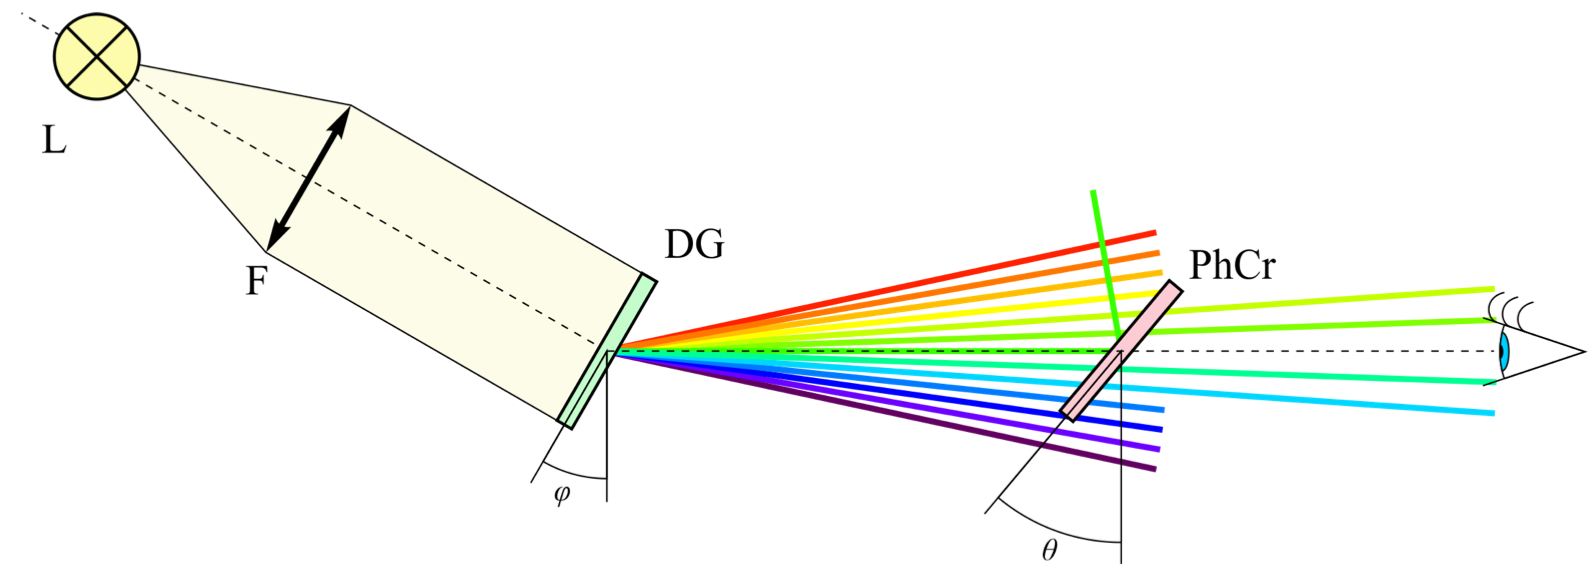
\includegraphics[width=1\linewidth]{Sch1.png}
		\caption{Схема экспериментальной установки для проведения спектральных исследований: (F) линза, (L) лампочка, расположенная в фокусе линзы, (DG) дифракционная решетка, (PhCr) фотонный кристалл.
		}
		\label{fig:3}
	\end{figure}
	Перейдём к рассмотрению зависимости между углами. Для начала посмотрим на график $\theta(\phi)$:
	\begin{figure}[H]
		\centering
		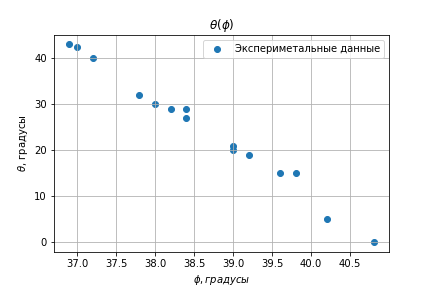
\includegraphics[width=0.75\linewidth]{Graph1.png}
		\caption{График с полученными данными.}
		\label{fig:4}
	\end{figure}
	Далее, используя формулу \ref{linear} получим линеаризованную зависимость, из которой легко найти параметры $D$ и $n$ кристалла.
	\begin{figure}[H]
		\centering
		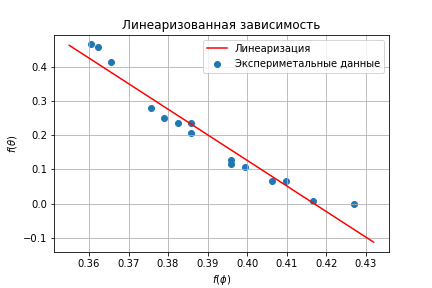
\includegraphics[width=0.75\linewidth]{Graph2.png}
		\caption{График с полученными данными.}
		\label{fig:5}
	\end{figure}
 Используя полученный полином первой степени и его пересечение с осями координат, очевидным образом получается:
	\begin{equation*}
 		D  \approx 220.5 \text{ нм}
	\end{equation*}
	\begin{equation*}
		n  \approx 1.55
	\end{equation*}
	\addcontentsline{toc}{section}{Второй эксперимент}
	\section*{Второй эксперимент}
	Производились замеры тока, протекающего через фотодиод в зависимости от угла, под которым находился кристалл. Ниже изображена схема установки:
		\begin{figure}[H]
		\centering
		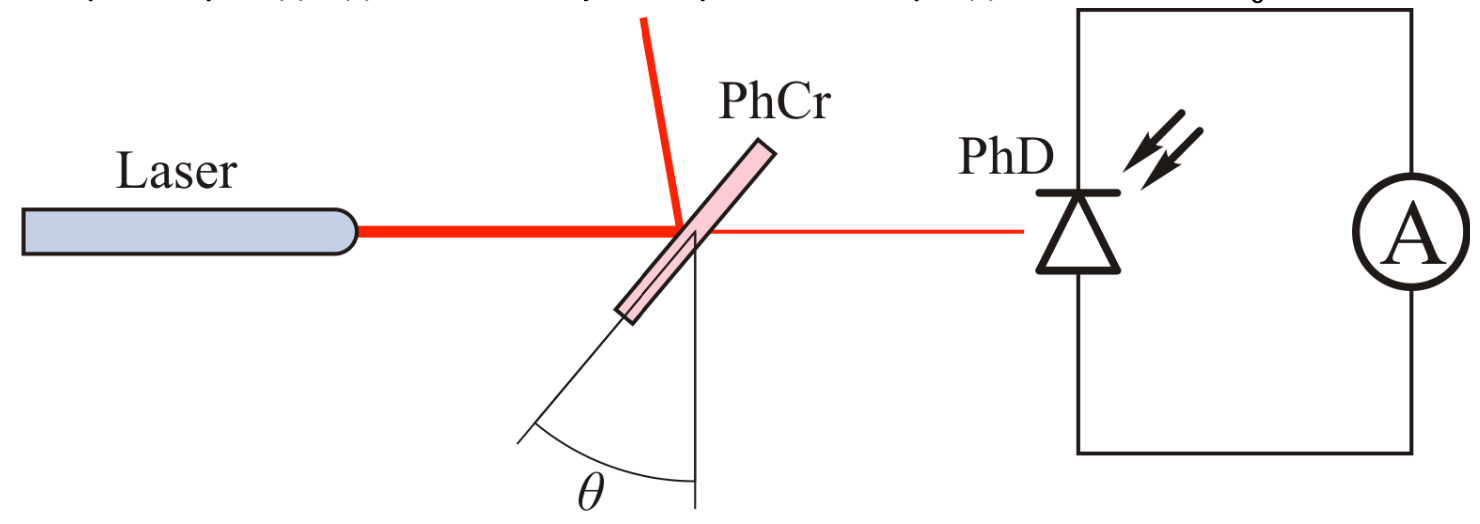
\includegraphics[width=0.9\linewidth]{Sch2.png}
		\caption{Схема второй установки.}
		\label{fig:6}
	\end{figure}
	Результаты измерений:
	\begin{figure}[H]
		\centering
		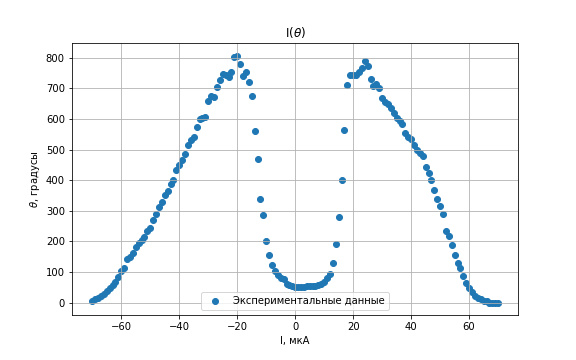
\includegraphics[width=0.85\linewidth]{Graph3.png}
		\caption{График с полученными данными.}
		\label{fig:7}
	\end{figure}
	Как можно заметить, при угле $\theta \approx 3^{\circ}$ ток достигает локального минимума. Ширина провала $\delta\theta \approx  29^{\circ}$
	Перепишем закон Брэгга-Снелла \ref{bg} для $\theta = 0^{\circ}$ и $\theta_{min} = 3^{\circ}$. Полученные выражения поделим друг на друга и получим:
	\begin{equation*}
		\frac{n}{\sqrt{n^{2}-\sin^{2}{\theta_{min}}}} = \frac{\lambda}{\lambda_{min}} 
	\end{equation*}
	Длина волны минимума пропускания:
	\begin{equation*}
		\lambda_{min} \approx 653 \text{ нм}
	\end{equation*}
	Считая что спектральная ширина минимума пропускания не зависит от угла падения, можно оценить разброс коэффициента преломления:
	Тогда можно выразить разницу показателей преломления:
	\begin{equation*}
	\Delta n = \frac{n\pi}{2} \frac{\Delta \lambda}{\lambda} \approx 0.14
	\end{equation*}
	\addcontentsline{toc}{section}{Вывод и дополнение}
	\section*{Вывод и дополнение}
	Были исследованы свойства твёрдых фотонных кристаллов. Экспериментальная зависимость угла падения от угла дифракции для минимальной длины волны пропускания достаточно близко совпадает с теоретической. Были найдены параметры фотонного кристалла, исследуемого в данном эксперименте: $D  \approx 220.5 \text{ нм}$, $n  \approx 1.55$. Также найдены параметры стоп-зоны образца: $\Delta n = \approx 0.14$, $\lambda_{min} \approx 653 \text{ нм}$. 
	
	Также, во время предыдущих работ, удалось воспользоваться спектрометром и получить следующие данные для этого фотонного кристалла:
	\begin{figure}[H]
		\centering
		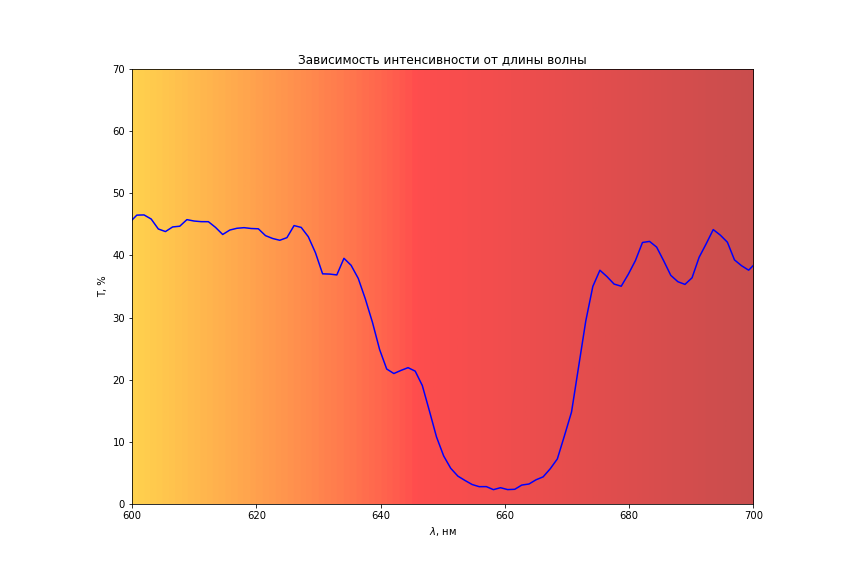
\includegraphics[width=0.85\linewidth]{Spec.png}
		\caption{Дополнение.}
		\label{fig:8}
	\end{figure}
	Как можно заметить, полученныев этой работе параметры стоп-зоны в целом сходятся с тем, что получено на спектрометре, различия могут быть вызваны в том числе и плохим состоянием образца и его некоторой неоднородностью.
	
	Таким образом, можно сказать, что в целом теория и эксперимент сходятся. Некоторые различия можно объяснить тем, что в вычислениях прибегали к приближениям (линериализация) и тем, что образец был последний целый (из нескольких имевшихся), однако имел несколько трещин, которые, скорее всего, внесли вклад в результат.
	\addcontentsline{toc}{section}{Список литературы}
	\begin{thebibliography}{9}
		\bibitem{metod} 
		Фотонные кристаллы.
		Методички к практикуму по оптике, 2021.
	\end{thebibliography}
\end{document}